% generated by Plantuml 1.2024.3       
\definecolor{plantucolor0000}{RGB}{255,192,203}
\definecolor{plantucolor0001}{RGB}{0,0,0}
\definecolor{plantucolor0002}{RGB}{173,216,230}
\definecolor{plantucolor0003}{RGB}{255,255,255}
\definecolor{plantucolor0004}{RGB}{24,24,24}
\definecolor{plantucolor0005}{RGB}{232,232,255}
\definecolor{plantucolor0006}{RGB}{255,234,213}
\definecolor{plantucolor0007}{RGB}{213,255,213}
\definecolor{plantucolor0008}{RGB}{255,232,232}
\definecolor{plantucolor0009}{RGB}{254,255,221}
\definecolor{plantucolor0010}{RGB}{238,238,238}
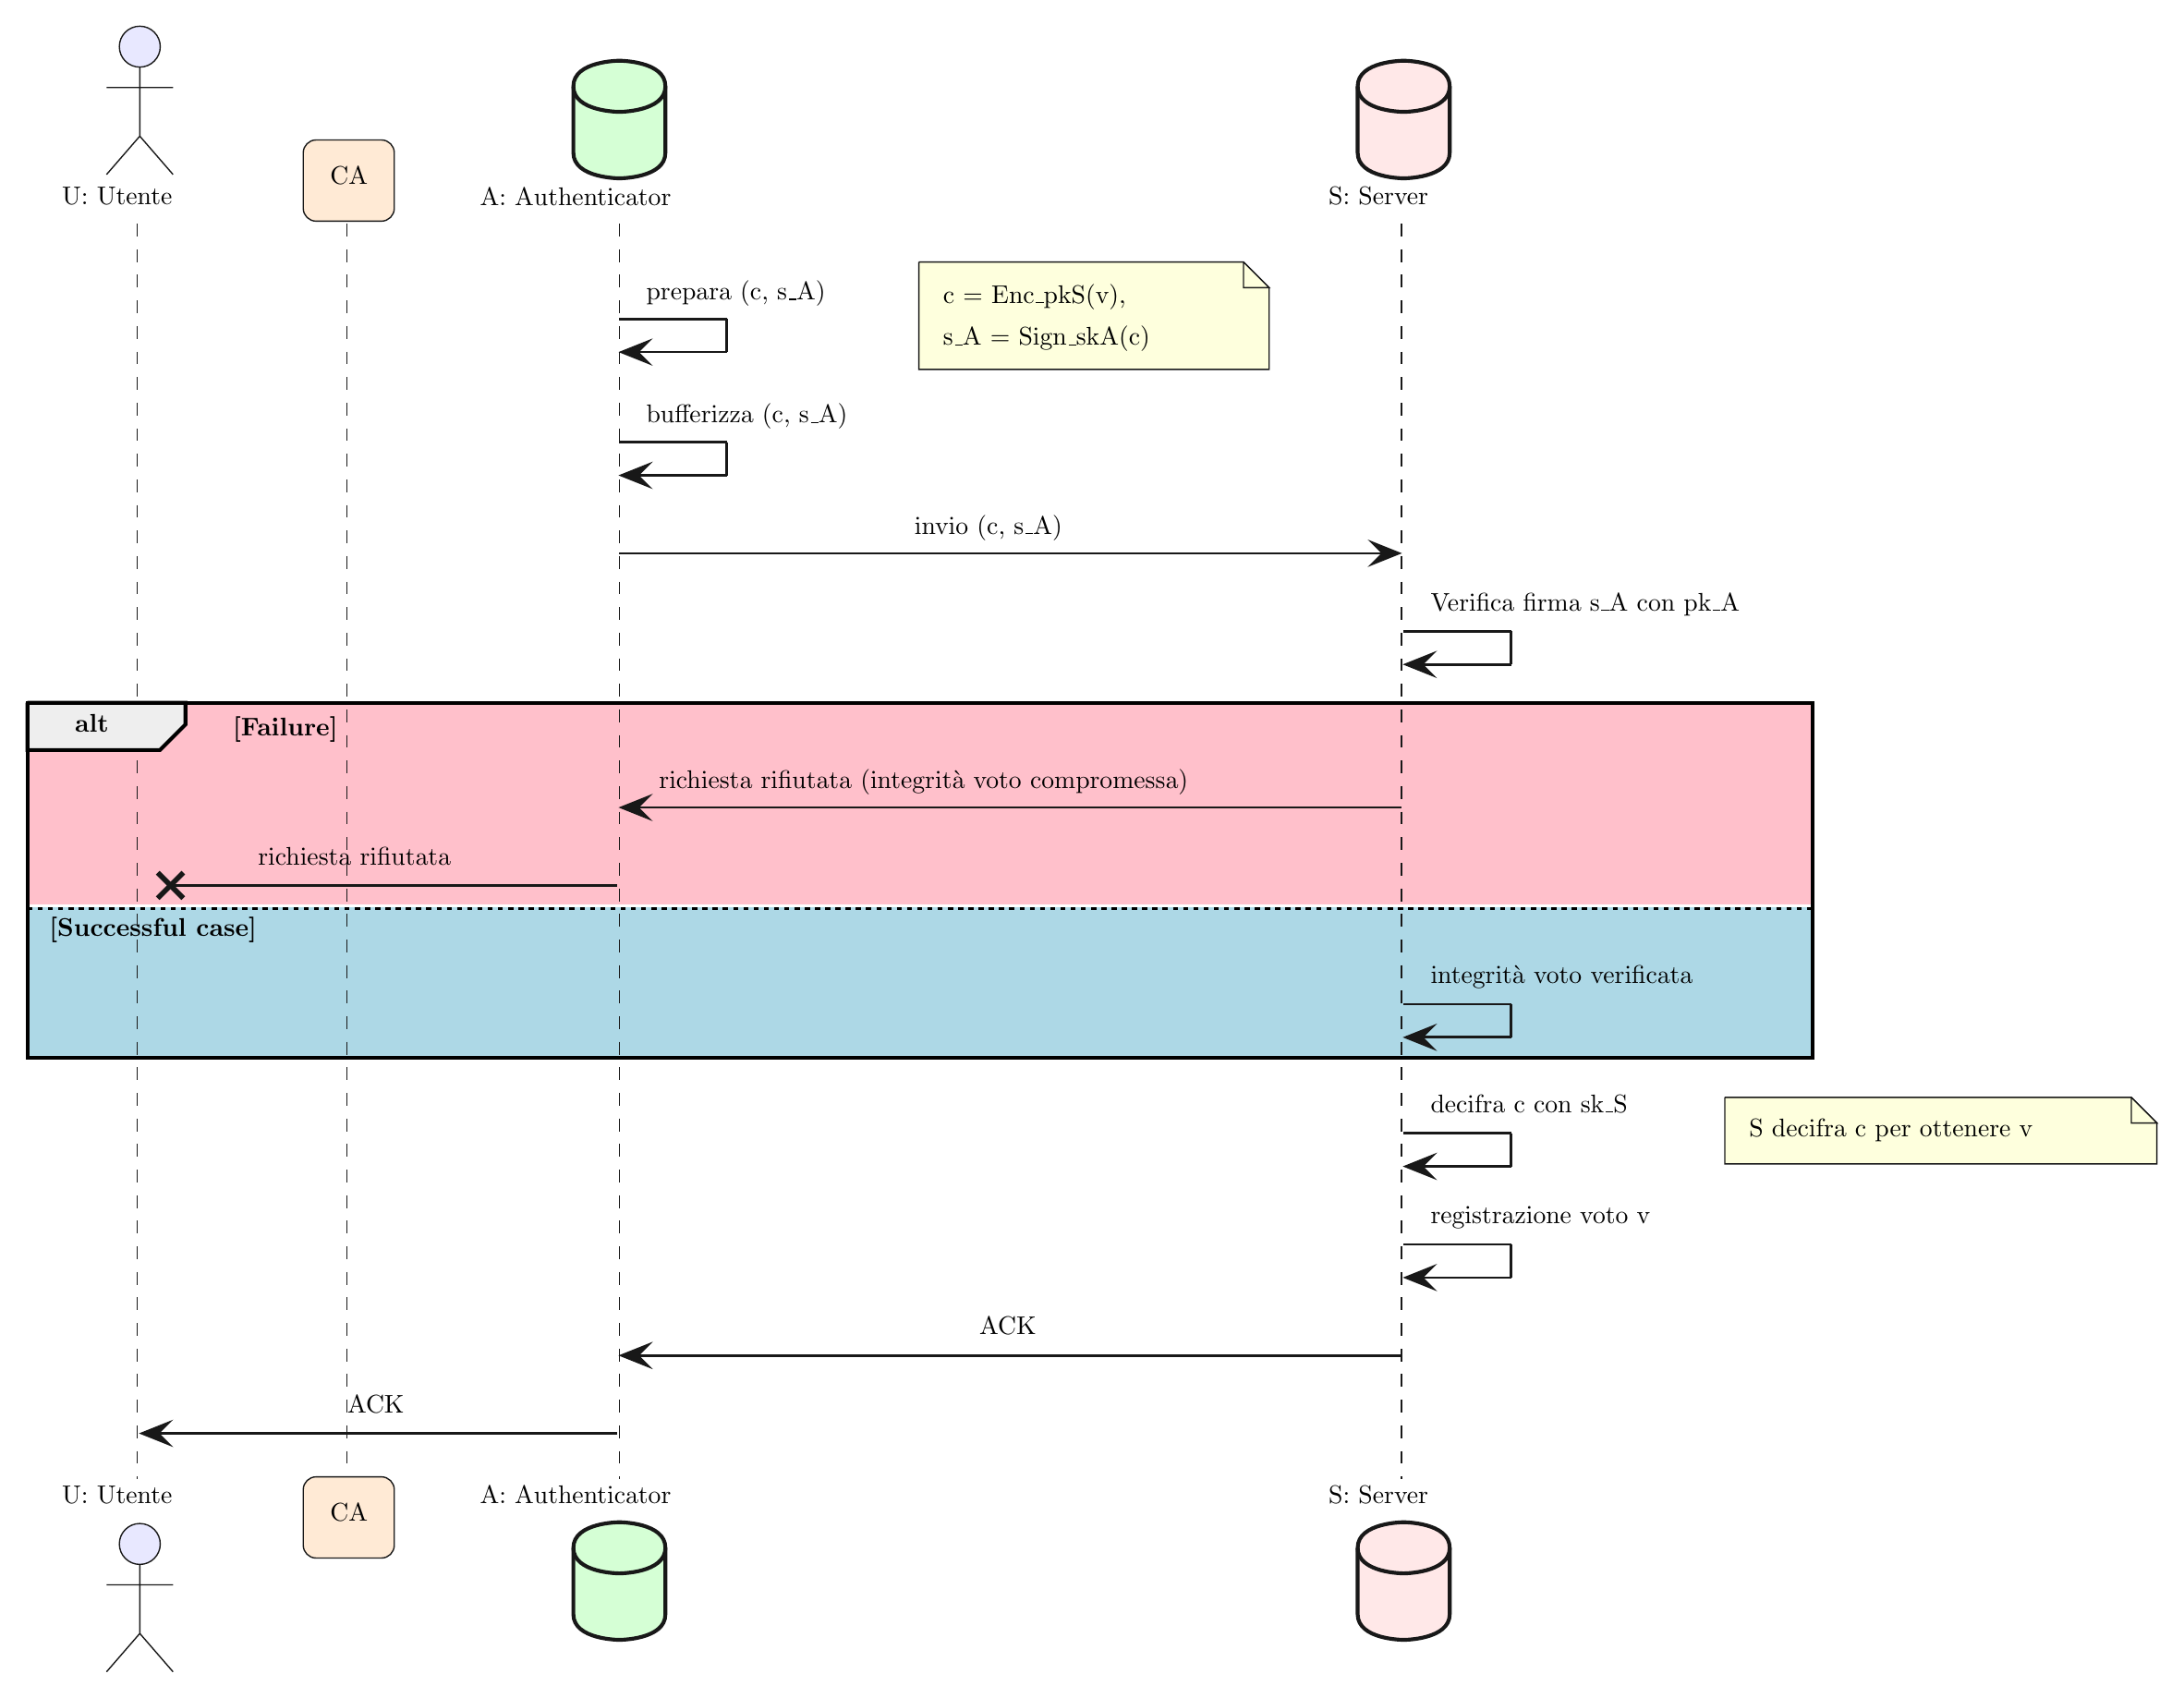
\begin{tikzpicture}[yscale=-1
,pstyle2/.style={color=plantucolor0004,line width=0.5pt,dash pattern=on 5.0pt off 5.0pt}
,pstyle3/.style={color=plantucolor0004,fill=plantucolor0005,line width=0.5pt}
,pstyle4/.style={color=plantucolor0004,line width=0.5pt}
,pstyle5/.style={color=plantucolor0004,fill=plantucolor0006,line width=0.5pt}
,pstyle6/.style={color=plantucolor0004,fill=plantucolor0007,line width=1.5pt}
,pstyle7/.style={color=plantucolor0004,line width=1.5pt}
,pstyle8/.style={color=plantucolor0004,fill=plantucolor0008,line width=1.5pt}
,pstyle9/.style={color=plantucolor0004,line width=1.0pt}
,pstyle10/.style={color=plantucolor0004,fill=plantucolor0004,line width=1.0pt}
,pstyle11/.style={color=plantucolor0004,fill=plantucolor0009,line width=0.5pt}
,pstyle14/.style={color=plantucolor0004,line width=2.0pt}
]
\draw[color=black,fill=plantucolor0000,line width=1.5pt] (10pt,270.1387pt) rectangle (708.1029pt,408.9961pt);
\draw[color=plantucolor0003,fill=plantucolor0002,line width=1.0pt] (10pt,349.5742pt) rectangle (708.1029pt,408.9961pt);
\draw[pstyle2] (53pt,82.7461pt) -- (53pt,573.9102pt);
\draw[pstyle2] (134.8615pt,82.7461pt) -- (134.8615pt,573.9102pt);
\draw[pstyle2] (241.4615pt,82.7461pt) -- (241.4615pt,573.9102pt);
\draw[pstyle2] (547.4168pt,82.7461pt) -- (547.4168pt,573.9102pt);
\node at (20pt,65pt)[below right,color=black]{U: Utente};
\draw[pstyle3] (53.9308pt,13.5pt) ellipse (8pt and 8pt);
\draw[pstyle4] (53.9308pt,21.5pt) -- (53.9308pt,48.5pt)(40.9308pt,29.5pt) -- (66.9308pt,29.5pt)(53.9308pt,48.5pt) -- (40.9308pt,63.5pt)(53.9308pt,48.5pt) -- (66.9308pt,63.5pt);
\node at (20pt,572.9102pt)[below right,color=black]{U: Utente};
\draw[pstyle3] (53.9308pt,599.1563pt) ellipse (8pt and 8pt);
\draw[pstyle4] (53.9308pt,607.1563pt) -- (53.9308pt,634.1563pt)(40.9308pt,615.1563pt) -- (66.9308pt,615.1563pt)(53.9308pt,634.1563pt) -- (40.9308pt,649.1563pt)(53.9308pt,634.1563pt) -- (66.9308pt,649.1563pt);
\draw[pstyle5] (117.8615pt,55pt) arc (180:270:5pt) -- (122.8615pt,50pt) -- (148.4615pt,50pt) arc (270:360:5pt) -- (153.4615pt,55pt) -- (153.4615pt,76.7461pt) arc (0:90:5pt) -- (148.4615pt,81.7461pt) -- (122.8615pt,81.7461pt) arc (90:180:5pt) -- (117.8615pt,76.7461pt) -- cycle;
\node at (124.8615pt,57pt)[below right,color=black]{CA};
\draw[pstyle5] (117.8615pt,577.9102pt) arc (180:270:5pt) -- (122.8615pt,572.9102pt) -- (148.4615pt,572.9102pt) arc (270:360:5pt) -- (153.4615pt,577.9102pt) -- (153.4615pt,599.6563pt) arc (0:90:5pt) -- (148.4615pt,604.6563pt) -- (122.8615pt,604.6563pt) arc (90:180:5pt) -- (117.8615pt,599.6563pt) -- cycle;
\node at (124.8615pt,579.9102pt)[below right,color=black]{CA};
\node at (183.4615pt,65pt)[below right,color=black]{A: Authenticator};
\draw[pstyle6] (223.5094pt,29pt) ..controls (223.5094pt,19pt) and (241.5094pt,19pt) .. (241.5094pt,19pt) ..controls (241.5094pt,19pt) and (259.5094pt,19pt) .. (259.5094pt,29pt) -- (259.5094pt,55pt) ..controls (259.5094pt,65pt) and (241.5094pt,65pt) .. (241.5094pt,65pt) ..controls (241.5094pt,65pt) and (223.5094pt,65pt) .. (223.5094pt,55pt) -- (223.5094pt,29pt);
\draw[pstyle7] (223.5094pt,29pt) ..controls (223.5094pt,39pt) and (241.5094pt,39pt) .. (241.5094pt,39pt) ..controls (241.5094pt,39pt) and (259.5094pt,39pt) .. (259.5094pt,29pt);
\node at (183.4615pt,572.9102pt)[below right,color=black]{A: Authenticator};
\draw[pstyle6] (223.5094pt,600.6563pt) ..controls (223.5094pt,590.6563pt) and (241.5094pt,590.6563pt) .. (241.5094pt,590.6563pt) ..controls (241.5094pt,590.6563pt) and (259.5094pt,590.6563pt) .. (259.5094pt,600.6563pt) -- (259.5094pt,626.6563pt) ..controls (259.5094pt,636.6563pt) and (241.5094pt,636.6563pt) .. (241.5094pt,636.6563pt) ..controls (241.5094pt,636.6563pt) and (223.5094pt,636.6563pt) .. (223.5094pt,626.6563pt) -- (223.5094pt,600.6563pt);
\draw[pstyle7] (223.5094pt,600.6563pt) ..controls (223.5094pt,610.6563pt) and (241.5094pt,610.6563pt) .. (241.5094pt,610.6563pt) ..controls (241.5094pt,610.6563pt) and (259.5094pt,610.6563pt) .. (259.5094pt,600.6563pt);
\node at (515.4168pt,65pt)[below right,color=black]{S: Server};
\draw[pstyle8] (530.2707pt,29pt) ..controls (530.2707pt,19pt) and (548.2707pt,19pt) .. (548.2707pt,19pt) ..controls (548.2707pt,19pt) and (566.2707pt,19pt) .. (566.2707pt,29pt) -- (566.2707pt,55pt) ..controls (566.2707pt,65pt) and (548.2707pt,65pt) .. (548.2707pt,65pt) ..controls (548.2707pt,65pt) and (530.2707pt,65pt) .. (530.2707pt,55pt) -- (530.2707pt,29pt);
\draw[pstyle7] (530.2707pt,29pt) ..controls (530.2707pt,39pt) and (548.2707pt,39pt) .. (548.2707pt,39pt) ..controls (548.2707pt,39pt) and (566.2707pt,39pt) .. (566.2707pt,29pt);
\node at (515.4168pt,572.9102pt)[below right,color=black]{S: Server};
\draw[pstyle8] (530.2707pt,600.6563pt) ..controls (530.2707pt,590.6563pt) and (548.2707pt,590.6563pt) .. (548.2707pt,590.6563pt) ..controls (548.2707pt,590.6563pt) and (566.2707pt,590.6563pt) .. (566.2707pt,600.6563pt) -- (566.2707pt,626.6563pt) ..controls (566.2707pt,636.6563pt) and (548.2707pt,636.6563pt) .. (548.2707pt,636.6563pt) ..controls (548.2707pt,636.6563pt) and (530.2707pt,636.6563pt) .. (530.2707pt,626.6563pt) -- (530.2707pt,600.6563pt);
\draw[pstyle7] (530.2707pt,600.6563pt) ..controls (530.2707pt,610.6563pt) and (548.2707pt,610.6563pt) .. (548.2707pt,610.6563pt) ..controls (548.2707pt,610.6563pt) and (566.2707pt,610.6563pt) .. (566.2707pt,600.6563pt);
\draw[pstyle9] (241.5094pt,119.9639pt) -- (283.5094pt,119.9639pt);
\draw[pstyle9] (283.5094pt,119.9639pt) -- (283.5094pt,132.9639pt);
\draw[pstyle9] (242.5094pt,132.9639pt) -- (283.5094pt,132.9639pt);
\draw[pstyle10] (252.5094pt,128.9639pt) -- (242.5094pt,132.9639pt) -- (252.5094pt,136.9639pt) -- (248.5094pt,132.9639pt) -- cycle;
\node at (248.5094pt,101.4854pt)[below right,color=black]{prepara (c, s\_A)};
\draw[pstyle11] (358.6419pt,97.7461pt) -- (358.6419pt,139.7461pt) -- (495.6419pt,139.7461pt) -- (495.6419pt,107.7461pt) -- (485.6419pt,97.7461pt) -- (358.6419pt,97.7461pt);
\draw[pstyle11] (485.6419pt,97.7461pt) -- (485.6419pt,107.7461pt) -- (495.6419pt,107.7461pt) -- (485.6419pt,97.7461pt);
\node at (364.6419pt,102.7461pt)[below right,color=black]{c = Enc\_pkS(v),};
\node at (364.6419pt,119.2246pt)[below right,color=black]{s\_A = Sign\_skA(c)};
\draw[pstyle9] (241.5094pt,168.1816pt) -- (283.5094pt,168.1816pt);
\draw[pstyle9] (283.5094pt,168.1816pt) -- (283.5094pt,181.1816pt);
\draw[pstyle9] (242.5094pt,181.1816pt) -- (283.5094pt,181.1816pt);
\draw[pstyle10] (252.5094pt,177.1816pt) -- (242.5094pt,181.1816pt) -- (252.5094pt,185.1816pt) -- (248.5094pt,181.1816pt) -- cycle;
\node at (248.5094pt,149.7031pt)[below right,color=black]{bufferizza (c, s\_A)};
\draw[pstyle10] (536.2707pt,207.6602pt) -- (546.2707pt,211.6602pt) -- (536.2707pt,215.6602pt) -- (540.2707pt,211.6602pt) -- cycle;
\draw[pstyle9] (241.5094pt,211.6602pt) -- (542.2707pt,211.6602pt);
\node at (353.3914pt,193.1816pt)[below right,color=black]{invio (c, s\_A)};
\draw[pstyle9] (548.2707pt,242.1387pt) -- (590.2707pt,242.1387pt);
\draw[pstyle9] (590.2707pt,242.1387pt) -- (590.2707pt,255.1387pt);
\draw[pstyle9] (549.2707pt,255.1387pt) -- (590.2707pt,255.1387pt);
\draw[pstyle10] (559.2707pt,251.1387pt) -- (549.2707pt,255.1387pt) -- (559.2707pt,259.1387pt) -- (555.2707pt,255.1387pt) -- cycle;
\node at (555.2707pt,223.6602pt)[below right,color=black]{Verifica firma s\_A con pk\_A};
\draw[color=black,fill=plantucolor0010,line width=1.5pt] (10pt,270.1387pt) -- (71.8pt,270.1387pt) -- (71.8pt,278.6172pt) -- (61.8pt,288.6172pt) -- (10pt,288.6172pt) -- (10pt,270.1387pt);
\draw[color=black,line width=1.5pt] (10pt,270.1387pt) rectangle (708.1029pt,408.9961pt);
\node at (25pt,271.1387pt)[below right,color=black]{\textbf{alt}};
\node at (86.8pt,272.1387pt)[below right,color=black]{\textbf{[Failure]}};
\draw[pstyle10] (252.5094pt,307.0957pt) -- (242.5094pt,311.0957pt) -- (252.5094pt,315.0957pt) -- (248.5094pt,311.0957pt) -- cycle;
\draw[pstyle9] (246.5094pt,311.0957pt) -- (547.2707pt,311.0957pt);
\node at (253.5094pt,292.6172pt)[below right,color=black]{richiesta rifiutata (integrità voto compromessa)};
\draw[pstyle14] (60.9308pt,336.5742pt) -- (70.9308pt,346.5742pt);
\draw[pstyle14] (60.9308pt,346.5742pt) -- (70.9308pt,336.5742pt);
\draw[pstyle9] (65.9308pt,341.5742pt) -- (240.5094pt,341.5742pt);
\node at (96.6571pt,323.0957pt)[below right,color=black]{richiesta rifiutata};
\draw[color=black,line width=1.0pt,dash pattern=on 2.0pt off 2.0pt] (10pt,350.5742pt) -- (708.1029pt,350.5742pt);
\node at (15pt,350.5742pt)[below right,color=black]{\textbf{[Successful case]}};
\draw[pstyle9] (548.2707pt,387.9961pt) -- (590.2707pt,387.9961pt);
\draw[pstyle9] (590.2707pt,387.9961pt) -- (590.2707pt,400.9961pt);
\draw[pstyle9] (549.2707pt,400.9961pt) -- (590.2707pt,400.9961pt);
\draw[pstyle10] (559.2707pt,396.9961pt) -- (549.2707pt,400.9961pt) -- (559.2707pt,404.9961pt) -- (555.2707pt,400.9961pt) -- cycle;
\node at (555.2707pt,369.5176pt)[below right,color=black]{integrità voto verificata};
\draw[pstyle9] (548.2707pt,438.4746pt) -- (590.2707pt,438.4746pt);
\draw[pstyle9] (590.2707pt,438.4746pt) -- (590.2707pt,451.4746pt);
\draw[pstyle9] (549.2707pt,451.4746pt) -- (590.2707pt,451.4746pt);
\draw[pstyle10] (559.2707pt,447.4746pt) -- (549.2707pt,451.4746pt) -- (559.2707pt,455.4746pt) -- (555.2707pt,451.4746pt) -- cycle;
\node at (555.2707pt,419.9961pt)[below right,color=black]{decifra c con sk\_S};
\draw[pstyle11] (673.8742pt,424.4961pt) -- (673.8742pt,450.4961pt) -- (842.8742pt,450.4961pt) -- (842.8742pt,434.4961pt) -- (832.8742pt,424.4961pt) -- (673.8742pt,424.4961pt);
\draw[pstyle11] (832.8742pt,424.4961pt) -- (832.8742pt,434.4961pt) -- (842.8742pt,434.4961pt) -- (832.8742pt,424.4961pt);
\node at (679.8742pt,429.4961pt)[below right,color=black]{S decifra c per ottenere v};
\draw[pstyle9] (548.2707pt,481.9531pt) -- (590.2707pt,481.9531pt);
\draw[pstyle9] (590.2707pt,481.9531pt) -- (590.2707pt,494.9531pt);
\draw[pstyle9] (549.2707pt,494.9531pt) -- (590.2707pt,494.9531pt);
\draw[pstyle10] (559.2707pt,490.9531pt) -- (549.2707pt,494.9531pt) -- (559.2707pt,498.9531pt) -- (555.2707pt,494.9531pt) -- cycle;
\node at (555.2707pt,463.4746pt)[below right,color=black]{registrazione voto v};
\draw[pstyle10] (252.5094pt,521.4316pt) -- (242.5094pt,525.4316pt) -- (252.5094pt,529.4316pt) -- (248.5094pt,525.4316pt) -- cycle;
\draw[pstyle9] (246.5094pt,525.4316pt) -- (547.2707pt,525.4316pt);
\node at (378.7641pt,506.9531pt)[below right,color=black]{ACK};
\draw[pstyle10] (64.9308pt,551.9102pt) -- (54.9308pt,555.9102pt) -- (64.9308pt,559.9102pt) -- (60.9308pt,555.9102pt) -- cycle;
\draw[pstyle9] (58.9308pt,555.9102pt) -- (240.5094pt,555.9102pt);
\node at (131.5941pt,537.4316pt)[below right,color=black]{ACK};
\end{tikzpicture}
